\documentclass[border=6pt]{standalone}
% ---------------------------------------------------------------------------
% tikzpreamble.tex -- shared by main.tex and by every standalone in tikz/
% ---------------------------------------------------------------------------
\usepackage{amsmath}
\usepackage{amssymb}
\usepackage{tikz}
\usepackage{circuitikz}
\usetikzlibrary{arrows.meta,calc,positioning,decorations.pathmorphing,decorations.pathreplacing,
                decorations.markings,patterns,angles,quotes,fit,
                shapes.geometric,shapes.misc,backgrounds,intersections}

\ctikzset{bipoles/length=0.85cm}
\ctikzset{resistors/scale=0.85}
\ctikzset{capacitors/scale=0.9}

\tikzset{
  wire/.style      = {line width=0.7pt},
  dashedwire/.style= {line width=0.7pt, densely dashed},
  term/.style      = {circle, draw, line width=0.6pt, fill=white,
                      inner sep=0pt, minimum size=4.5pt},
  node dot/.style  = {circle, fill=black, inner sep=0pt, minimum size=4pt},
  boxlabel/.style  = {font=\sffamily\small},
  annot/.style     = {font=\small, align=left},
  phasor/.style    = {-{Stealth[length=3.2mm,width=2.2mm]}, line width=1.1pt},
  thinphasor/.style= {-{Stealth[length=2.6mm,width=1.8mm]}, line width=0.7pt},
  axis line/.style = {-{Stealth[length=2.6mm,width=1.8mm]}, line width=0.6pt},
  guide/.style     = {densely dashed, line width=0.4pt, gray},
}
\usepackage{siunitx}

\begin{document}
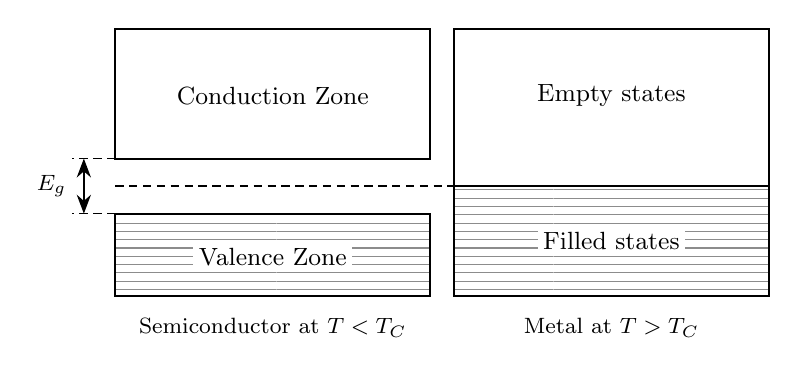
\begin{tikzpicture}[every node/.style={font=\small}]
  % ---------------- semiconducting side ----------------------------------
  \draw[wire] (0,1.75) rectangle (4.0,3.4);
  \node at (2.0,2.55) {Conduction Zone};
  \draw[wire,pattern=horizontal lines,pattern color=black!45] (0,0) rectangle (4.0,1.05);
  \draw[wire] (0,0) rectangle (4.0,1.05);
  \node[fill=white,inner sep=2pt] at (2.0,0.5) {Valence Zone};

  % ---------------- metallic side ----------------------------------------
  \draw[wire] (4.3,1.4) rectangle (8.3,3.4);
  \node at (6.3,2.55) {Empty states};
  \draw[wire,pattern=horizontal lines,pattern color=black!45] (4.3,0) rectangle (8.3,1.4);
  \draw[wire] (4.3,0) rectangle (8.3,1.4);
  \node[fill=white,inner sep=2pt] at (6.3,0.7) {Filled states};

  % ---------------- Fermi level & gap ------------------------------------
  \draw[densely dashed,line width=0.8pt] (0,1.4) -- (8.3,1.4);
  \draw[guide,black] (0,1.05) -- (-0.55,1.05);
  \draw[guide,black] (0,1.75) -- (-0.55,1.75);
  \draw[{Stealth[length=2.4mm]}-{Stealth[length=2.4mm]},line width=0.6pt]
        (-0.4,1.05) -- (-0.4,1.75);
  \node[anchor=east,font=\footnotesize] at (-0.5,1.4) {$E_g$};

  \node[anchor=north,font=\footnotesize] at (2.0,-0.15) {Semiconductor at $T<T_C$};
  \node[anchor=north,font=\footnotesize] at (6.3,-0.15) {Metal at $T>T_C$};
\end{tikzpicture}
\end{document}
